\documentclass{article}
\usepackage{blindtext}
\usepackage[utf8]{inputenc}
\usepackage{amsmath,bm}
\usepackage{amstext}
\usepackage{amsfonts}
\usepackage{amsmath}
\usepackage{multirow}
\usepackage{enumerate}
\usepackage{xeCJK}
\setCJKmainfont{STKaiti}
\usepackage{algorithm}
\usepackage{algorithmic}
\renewcommand{\algorithmicrequire}{ \textbf{输入:}} %Use Input in the format of Algorithm
\renewcommand{\algorithmicensure}{ \textbf{输出:}} %UseOutput in the format ofAlgorithm
\usepackage{graphicx}
%超链接
\usepackage[colorlinks, linkcolor=blue]{hyperref}
%tabular
\usepackage{booktabs}
%java代码模板
 \usepackage{listings}
\usepackage{color}
\usepackage{xcolor}
\definecolor{dkgreen}{rgb}{0,0.6,0}
\definecolor{gray}{rgb}{0.5,0.5,0.5}
\definecolor{mauve}{rgb}{0.58,0,0.82}
\lstset{frame=tb,
	language=Java,
	aboveskip=3mm,
	belowskip=3mm,
	showstringspaces=false,
	columns=flexible,
	basicstyle = \ttfamily\small,
	numbers=none,
	numberstyle=\tiny\color{gray},
	keywordstyle=\color{blue},
	commentstyle=\color{dkgreen},
	stringstyle=\color{mauve},
	breaklines=true,
	breakatwhitespace=true,
	tabsize=3
}

\title{MapReduce大数据实验四—MyJoin\_Hive}
\author{卢庆宁 MG20330040\\邹德润 MG20330094\\徐业婷 MF20330097\\陈轶洲 MF20330010}
\begin{document}
	\maketitle
	\numberwithin{equation}{section}

\section{实验任务描述}
使用 MapReduce 完成两张表的 join 操作。实验数据在 hdfs://master001:9000/data/hive\_myjoin 目录下。单机测试可以使用
FTP“实验要求”目录下的测试数据集。
\begin{enumerate}[1)]
	\item 输入数据为 order.txt 和 product.txt;
	\item 先将这两个文件通过使用 MapReduce 进行 join 操作,将结果输出到 HDFS 的个
	人目录上;
	\item 进入 SQL On Hadoop 页面,使用 Hive 建表管理上一步输出的结果;
	\item 最后在 Hive 上通过 show tables 能查看到名为 orders 的表,并且通过 select
	语句能查出内容。
\end{enumerate}

\section{实验设计}

\subsection{实验环境}
\begin{table}[htbp]
	\centering
	\begin{tabular}{cccccc}
		\toprule    Linux环境 & Java版本  & Hadoop版本 & IDE& Maven&集群名称 \\
		\midrule   Ubuntu18.04 & jdk1.8 & hadoop2.7.1 &ItelliJ IDEA(mac os)&maven3.6&2021st20\\   
		\bottomrule   
	\end{tabular}  
\end{table}

\subsection{实验任务流程}
\begin{enumerate}[1)]
	\item 小组开会进行任务的分配,伪代码的设计,并按照讨论得出的思路进行实现
	\item 小组成员进行具体代码的编写,利用maven管理项目,生成jar包,进行本地测试
	\item 进行集群的测试,查看结果,撰写实验报告
\end{enumerate}


\section{实验具体实现}
本次实验的要求是将两张表中的数据进行连接,我们的实现借鉴了课堂ppt与书本代码的思路。

\subsection{设计思路}
Mapper的输入为待合并的两张表中的每一行数据,输出的Key为标记了来源表的Join的字段内容,Value为原表的记录。\\
Reducer在接收到同一个Key的记录后遍历Values,并根据Key中不同的来源表标签执行不同操作:“product”——将该条记录加入到一个List中;"order"——遍历上一种情况生成的List,对List中的每一条来自产品的数据生成join结果并输出。(在区分复合键时进行二次排序,确保分类后product记录出现在order记录之前。)

\subsection{覆写}
进行了Map类和Reduce类的重写,并实现了Partitioner、WritableComparable和WritableComparator方法。

\subsection{TaggedKey复合键}

\subsubsection{实现思路}
将两张表连接利用的是他们记录中相同的product\_id,除此以外我们还需要标记这条数据来自哪个文件,故需要设计一个Tag(IntWritable类型)。将这二者结合得到<Text product\_id, IntWritable Tag>,就是本实验中需要使用的复合键。\\
为了定义复合键我们还需要实现WritableComparable接口:利用二次排序,首先比较product\_id,若不同则返回比较结果,若相同则继续比较Tag,并返回Tag的比较结果。
\subsubsection{实际代码}

\begin{lstlisting}
	//WritableComparable
	public static class TaggedKey implements WritableComparable<TaggedKey>{
		private Text joinKey = new Text();//product_id
		private IntWritable tag = new IntWritable();//Tag
		//implement compareTo()
		public int compareTo(TaggedKey taggedKey){
			//compare product_id
			int compareValue = joinKey.compareTo(taggedKey.getJoinKey());
			//if product_id equals, then compare Tag
			if (compareValue == 0){
				compareValue = tag.compareTo(taggedKey.getTag());
			}
			return compareValue;
		}
		public void readFields(DataInput in) throws IOException{
			joinKey.readFields(in);
			tag.readFields(in);
		}
		//implement write() and set()
		public void write(DataOutput out) throws IOException{
			joinKey.write(out);
			tag.write(out);
		}
		public void set(String joinKey, int tag){
			this.joinKey.set(joinKey);
			this.tag.set(tag);
		}
		//implement get() to get product_id or Tag
		public Text getJoinKey(){
			return joinKey;
		}
		public IntWritable getTag(){
			return tag;
		}
	}
\end{lstlisting}



\subsection{Map类}

\subsubsection{输入输出格式}

\begin{table}[htbp]
	\centering
	\begin{tabular}{cc}
		\toprule    输入 & <LongWritable, Text> \\
		\midrule   输出 & <TaggedKey, Text>=<<pid,sourcefile>, record> \\ 
		\bottomrule   
	\end{tabular}  
\end{table}

\subsubsection{实现思路}
首先获取文件名并去除文件名后缀(得到“product”或“order”),然后对内容进行读取,此时读取的是文件的每一行。根据来源文件设置Tag(IntWritable类型):来自product的数据的Tag置为1,来自order的数据的Tag置为2。根据不同Tag就能从文本中提取不同来源文件的product\_id。将复合键<Text product\_id, IntWritable Tag>作为Key,数据Text value作为value输出。

\subsubsection{实际代码}

\begin{lstlisting}
	//Mapper
	public static class DataMapper extends Mapper<LongWritable, Text, TaggedKey, Text>{
		@Override
		protected void map(LongWritable key, Text value, Context context)
		throws IOException, InterruptedException{
			String[] columns = value.toString().split(" ");
			TaggedKey taggedKey = new TaggedKey();
			//setting <key, value> depends on filename
			FileSplit fileSplit = (FileSplit)context.getInputSplit();
			String fileName = fileSplit.getPath().getName();
			if(fileName.startsWith("product")){
				//columns[0] is pid in product.txt, tag is 1
				taggedKey.set(columns[0], 1);
				context.write(taggedKey, value);
			} else if(fileName.startsWith("order")){
				//columns[2] is pid in order.txt, tag is 2
				taggedKey.set(columns[2], 2);
				context.write(taggedKey, value);
			}
		}
	}
\end{lstlisting}

\subsection{Partitioner类}

\subsubsection{实现思路}
默认情况下,Hadoop会对Key进行哈希,以保证相同的Key会分配到同一个Reducer中。由于我们改变了Key的结构,因此需要重新编 写分区函数:只利用product\_id分区,而忽略Tag的不同。这样可以使不同文件中具有相同product\_id的记录分到一个Reducer中。

\subsubsection{实际代码}
\begin{lstlisting}
	 //Partitioner
	public static class TaggedPartitioner extends Partitioner<TaggedKey, Text>{
		@Override
		public int getPartition(TaggedKey taggedKey, Text text, int numPartition){
			//partition TaggedKey by accessing product_id's hash
			return taggedKey.getJoinKey().hashCode()%numPartition;
		}
	}
\end{lstlisting}

\subsection{WritableComparator类}

\subsubsection{实现思路}
同Partitioner,调用reduce函数需要传入同一个Key的所有记录,这就需要重新定义分组函数.

\subsubsection{实际代码}
\begin{lstlisting}
	//WritableComparator
	public static class TaggedJoinComparator extends WritableComparator{
		
		public  TaggedJoinComparator(){
			super(TaggedKey.class, true);
		}
		
		@SuppressWarnings("rawtypes")
		@Override
		public int compare(WritableComparable a, WritableComparable b){
			TaggedKey key1 = (TaggedKey) a;
			TaggedKey key2 = (TaggedKey) b;
			return key1.getJoinKey().compareTo(key2.getJoinKey());
		}
	}
\end{lstlisting}

\subsection{Reduce类}

\subsubsection{输入输出格式}

\begin{table}[htbp]
	\centering
	\begin{tabular}{cc}
		\toprule    输入 & <TaggedKey, Iterable<Text>>=<<pid,sourcefile>,records[]> \\
		\midrule   输出 & <NullWritable, Iterable>=<records[]> \\ 
		\bottomrule   
	\end{tabular}  
\end{table}

\subsubsection{实现思路}
因为partitioner仅按照不同的product\_id划分,所以对于一个Reducer,包含了text和不同的Tag,因此我们需要区分每条记录来自product还是order。
设置全局变量List<String>products,遍历记录,当这条记录来自produc时,我们将该Text转换成String并存入products中;当这条记录来自order时,我们遍历products,将其中每条product记录与该order记录进行join操作并输出。\\
因为最终只要求输出连接后的记录,所以将输出的Key置为NullWritable。

\subsubsection{实际代码}

\begin{lstlisting}
	 //Reducer
	public static class JoinReducer extends Reducer<TaggedKey, Text, NullWritable, Text>{
		List<String> products = new ArrayList<String>();//save records from product
		@Override
		protected void reduce(TaggedKey key, Iterable<Text> values, Context context)
		throws IOException, InterruptedException {
			for (Text value : values) {
				switch (key.getTag().get()) {
					case 1: // product
					products.add(value.toString());//add to products
					break;
					case 2: // order
					String[] order = value.toString().split(" ");
					for (String productString : products) {
						String[] product = productString.split(" ");
						//join data
						if(order[2].equals(product[0])) {
							List<String> output = new ArrayList<String>();
							output.add(order[0]);
							output.add(order[1]);
							output.add(order[2]);
							output.add(product[1]);
							output.add(product[2]);
							output.add(order[3]);
							//output
							context.write(NullWritable.get(), new Text(StringUtils.join(output, " ")));
						}
					}
					break;
					default:
					assert false;
				}
			}
		}
	}
\end{lstlisting}


\section{实验运行与结果分析}

\subsection{配置管理}
利用maven进行包的依赖项的添加和项目的打包管理。生成jar包类型。具体见pom.xml文件。

\subsection{生成jar包运行结果}
输出结果文件在 HDFS 上的路径 :$/user/2021st20/output3$ 。两张表连接生成的结果文件为part-r-00000,显示如下:
\begin{figure}[H]
	\centering
	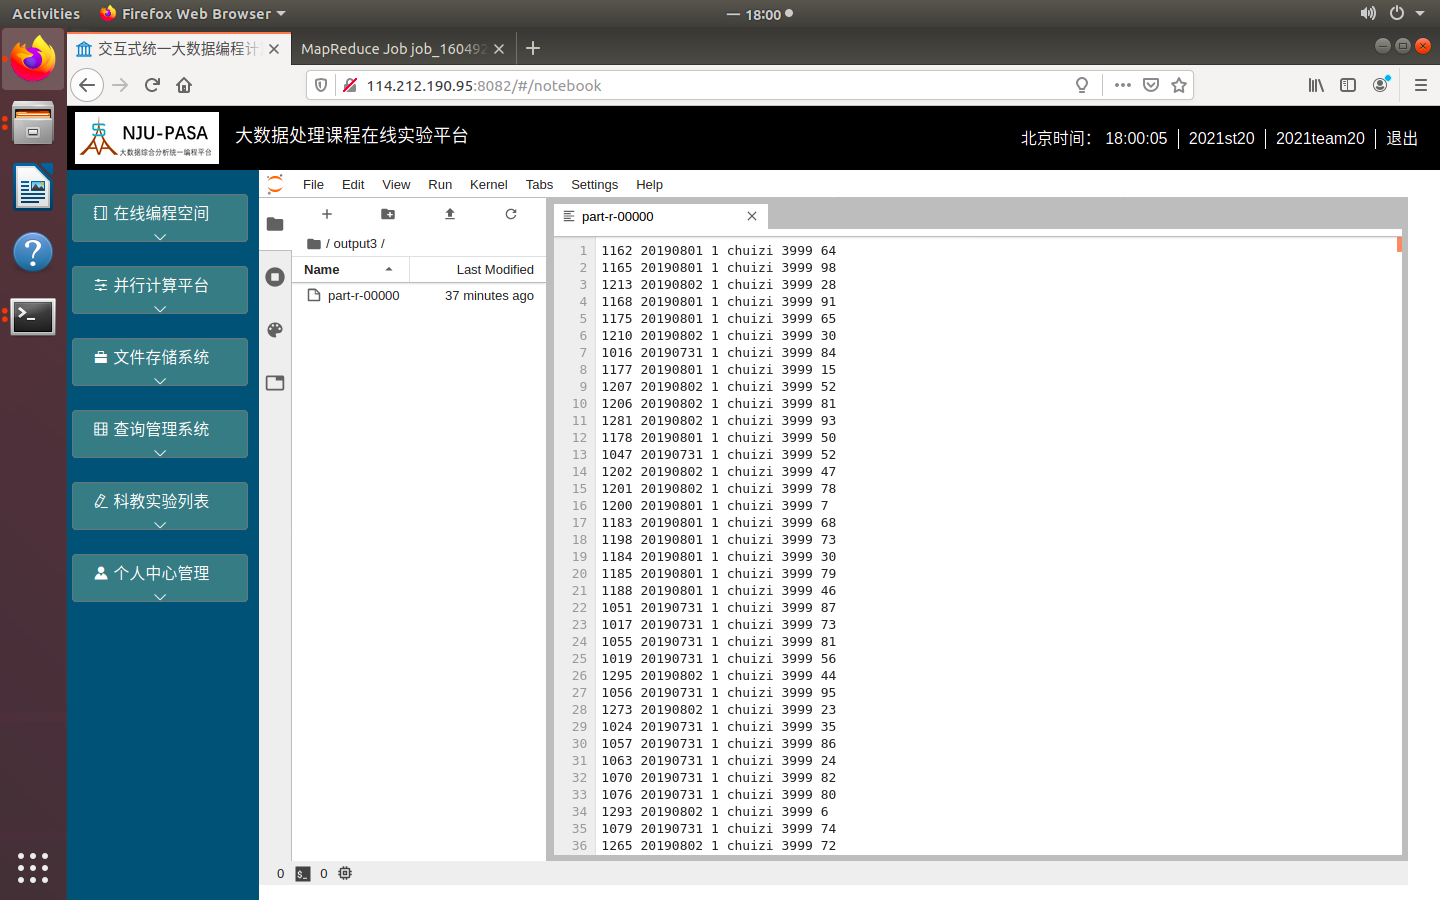
\includegraphics[scale=0.2]{output.png}
\end{figure}

\subsection{Hive输出结果文件}
利用上一小节生成的part-r-00000文件建表,在SQL On Hadoop中输入如下指令:\\
 create table 2021st20\_orders(id int,order\_date string,pid string,name string,price int,num int) row format delimited fields terminated by '  ' location '/user/2021st20/output3/'; \\
 利用select语句查看此表:
 \begin{figure}[H]
 	\centering
 	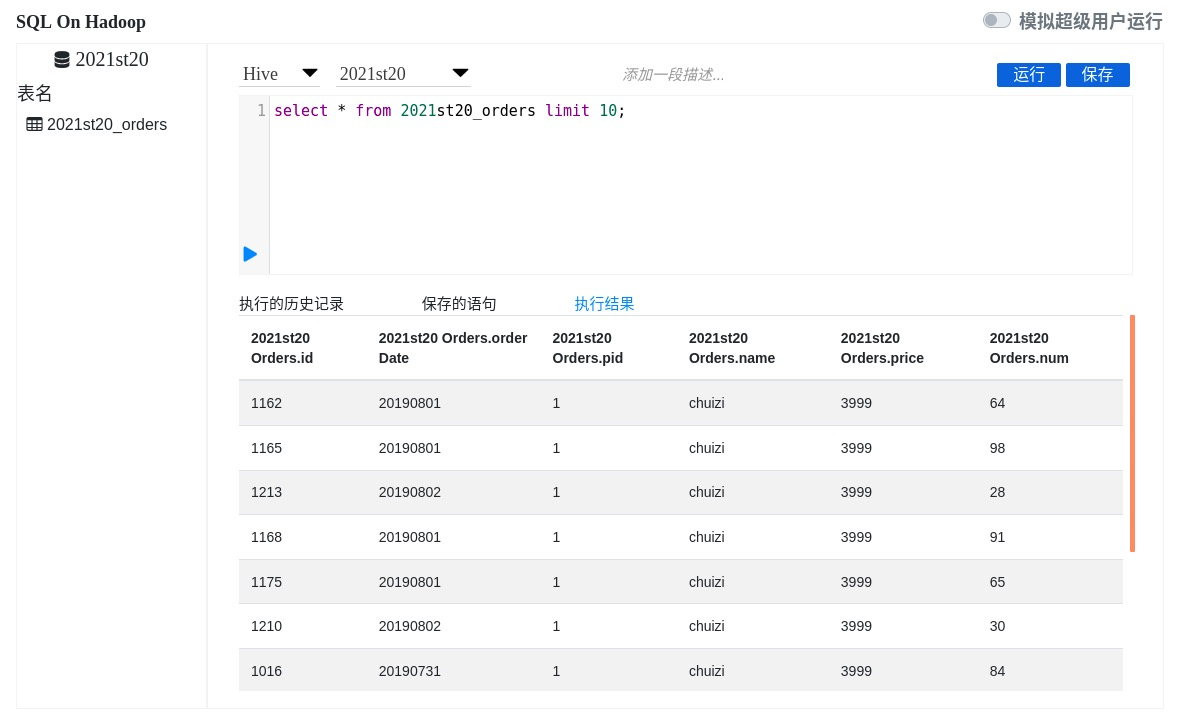
\includegraphics[scale=0.25]{hive.jpg}
 \end{figure}
 
\subsection{Web-ui结果}
Job ID: job\_1604923458283\_0255 

 \begin{figure}[H]
	\centering
	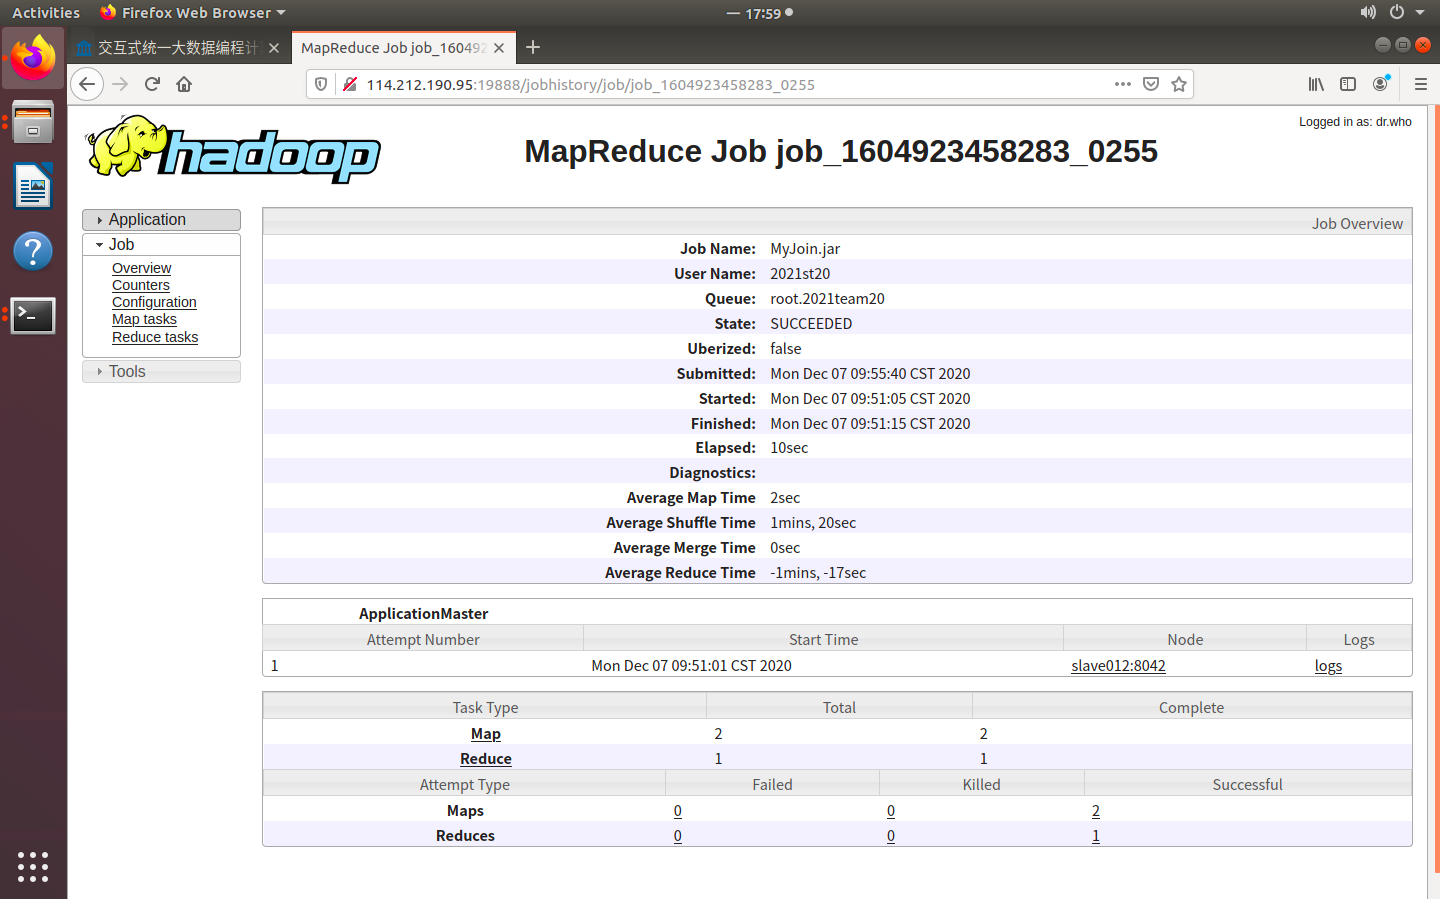
\includegraphics[scale=0.2]{webui.png}
\end{figure}

\section{实验总结和参考}

\subsection{实验总结}

\begin{enumerate}[1)]
	\item 本次实现通过自己实现hadoop的mapreduce程序,了解了对于map-reduce程序编写,懂得了设计的重要性,并且通过maven管理了项目,使得项目的打包运行更方便;
	\item 同时小组通过开会等,分工明确,互相帮助,共同完成这次实验,体现了团队协作的重要性,在一个项目中团队精神是不可缺少的;
	\item 在实验中遇到了并行问题,通过询问助教后得到解决。因为hadoop不保证一个reducer只执行一次reduce,所以设计时需要格外注意保护各个变量的信息;
	\item 最后感谢助教和其他同学对本次实验提供的帮助。
\end{enumerate}

\subsection{实验参考}

\begin{enumerate}[1)]
	\item  \href{http://shzhangji.com/cnblogs/2015/01/13/understand-reduce-side-join/}{深入理解Reduce-side Join}
	\item \href{https://blog.csdn.net/H_X_P_/article/details/106071511}{Hadoop-MapReduce-Reduce阶段调用reduce()方法过程源
	}
\end{enumerate}

\end{document}
